\documentclass{article}
\usepackage{amsthm}
\usepackage{graphicx}
\usepackage{subfig}
\usepackage{physics}
\graphicspath{ {figures/} }

\title{The Tight Binding Model}
\author{Caitlin Carnahan}
\begin{document}
\maketitle
\begin{abstract}
This document is intended as a detailed review of covalent bonding and the Tight Binding (LCAO) model in preparation for study of monolayer and bilayer graphene.
\end{abstract}
\section{Covalent Bonding}
Graphene is composed of hexagonally-shaped links of carbon atoms, each of which is linked to three other carbon atoms when the hexagons are tiled. These carbon atoms are linked together by covalent bonds.
The purpose of this section is to review the fundamental concepts of covalent bonding, as well as the properties of the carbon atom itself. \par
Carbon is the chemical element with atomic number 6 - that is, there are six protons found in the nucleus of a Carbon atom. The ground-state electron configuration of Carbon is $1s^{2}2s^{2}2p^{2}$. However, when in the presence of other atoms,
it is sometimes energetically favorable to promote one electron into the $2p$ orbital - the energy cost of moving into this excited state is offset by the energy gained from covalent bonding. \par
In the case of graphene, carbon atoms exibit $sp^{2}$ hybridization wherein two $2p$ orbitals, conventionally chosen as $2p_{x}$ and $2p_{y}$, form a superposition with the $2s$ orbital. The result is three coplanar orbitals separated by $120^{\circ}$.
The remaining $2p_{z}$ orbital lies perpendicular to the coplanar hybridized orbitals. Sheets of graphene are formed by planes of carbon atoms bonding via the hybridized orbitals, but this leaves the perpendicular $2p_{z}$ orbital free. \par
We now turn our attention to the nature of covalent bonding in graphene. What follows is a description of covalent bonding that closely follows that presented in \cite{oxford}. As a simple model, we can demonstrate the energetically favorable effects
produced by covalent bonding if we imagine an atom as a potential well for an electron - specifically, we model an atom as an infinite square well.
\begin{figure}[h]
\centering
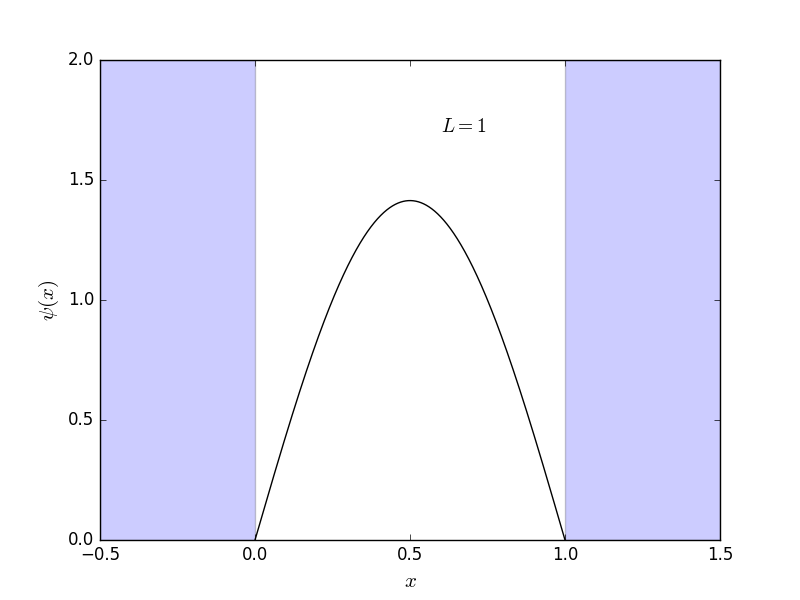
\includegraphics[scale=.5]{figure_1}
\caption{The ground state $\psi(x)$ for the case $L = 1$.}
\end{figure}
The ground state energy for a single electron in the infinite square well is given by: $$E = \frac{\pi^{2}\hbar^{2}}{2mL^{2}}$$
and the ground state solution is $$\psi(x) = \sqrt{\frac{2}{L}}sin\left (\frac{\pi x}{L}\right )$$ If we have two such atoms and we bring them close enough together, a single electron can be found in the shared space produced by doubling the well width. If the well width is doubled
to $2L$, then the ground state energy becomes $$E = \frac{\pi^{2}\hbar^{2}}{2m(2L)^{2}}$$ Therefore, doubling the well width decreases the ground state energy by a factor of 4.
\begin{figure}[h]
\centering
\subfloat{{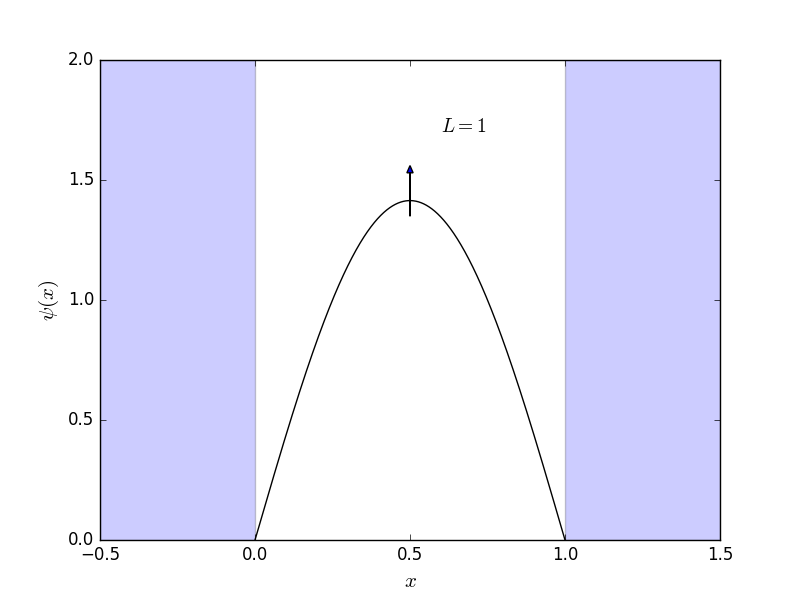
\includegraphics[scale=.28]{figure_2_up}}}%
\qquad
\subfloat{{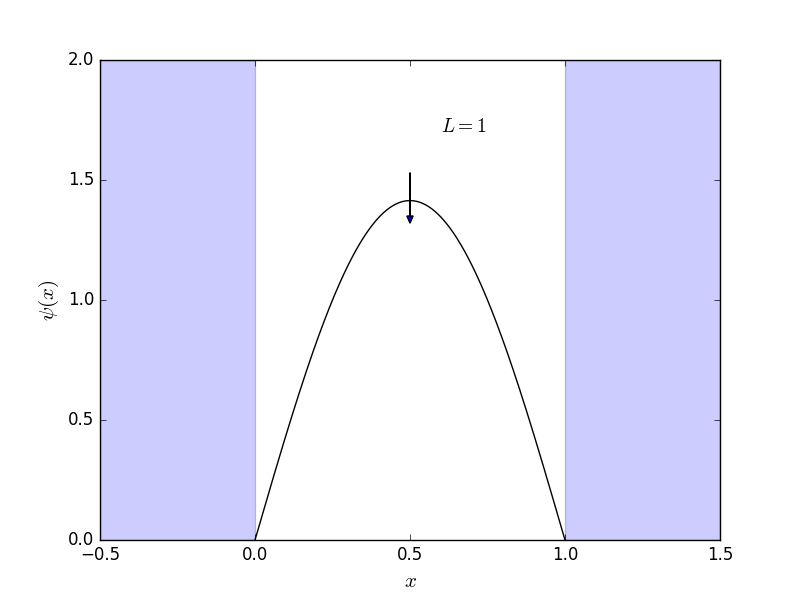
\includegraphics[scale=.28]{figure_2_down}}}%
\caption{The individual ground state $\psi(x)$ for the case $L = 1$ shown for each atom - one with elecron spin up and the other with spin down.}
\end{figure}

This simple model demonstrates the motivation for covalent bonding: delocalizing the electron is energetically favorable
because the new ground state (the \emph{bonding} orbital) is lower in energy than the original ground state. This principle holds even when considering one electron on each of the two atoms -- both electrons can occupy the new lower-energy bonding orbital if they have opposite spin states. However, covalent bonding is not energetically favorable in every situation - \emph{antibonding} orbitals can be produced that offset the decrease in energy due to the bonding orbital.

\begin{figure}[h]
\centering
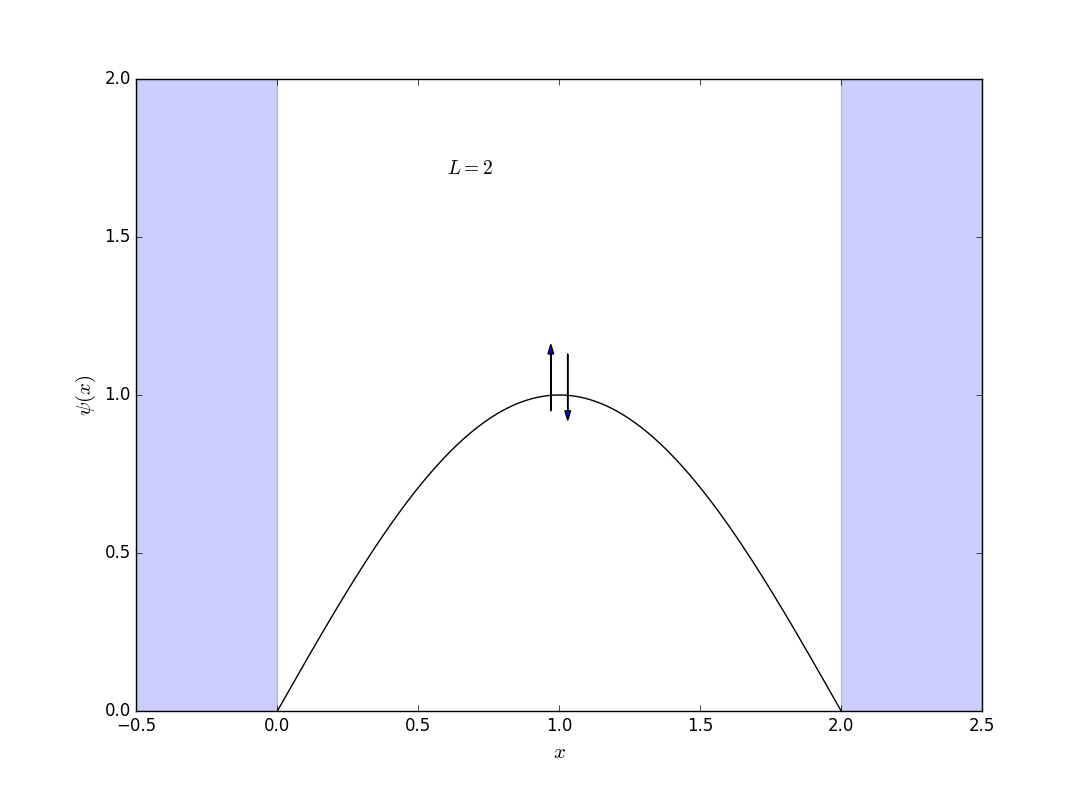
\includegraphics[scale=.4]{figure_2_both}
\caption{The new ground state $\psi(x)$ for the case $L = 2$ with two spin states.}
\end{figure}

\section{Tight Binding Model}
\subsection{Introduction: Two Hydrogen Atoms}
We begin our discussion of the tight binding model by considering a simple system of two hydrogen atoms. Each hydrogen atom has a single electron orbiting its nucleus. Individually,
the ground state of an electron orbiting a hydrogen nucleus has the form
$$ \psi(r) = \frac{1}{\sqrt{\pi}a_{0}^{3/2}}e^{-r/a_{0}}$$
and exhibits the following radial probability density, plotted in Figure 4 with $a_{0} = 1$.
$$ P(r) = \int_{V} \left | \psi(r)\right |^{2} rsin(\theta)drd\theta d\phi= \left ( \frac{4r^{2}}{a_{0}^3}\right )e^{-2r/a_{0}}$$
In the region $0 \geq r \leq 2a_{0}$, this probability distribution is roughly equivalent to the infinite square well probability distribution, also shown in Figure 4. So, we can
clearly model the hydrogen atom as a square potential well.
\begin{figure}[h]
\centering
\subfloat{{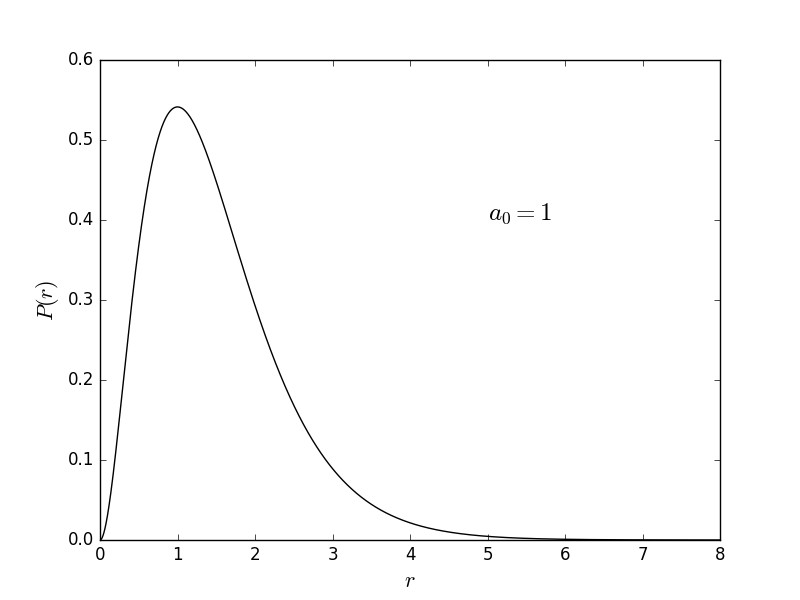
\includegraphics[scale=.28]{figure_4}}}%
\qquad
\subfloat{{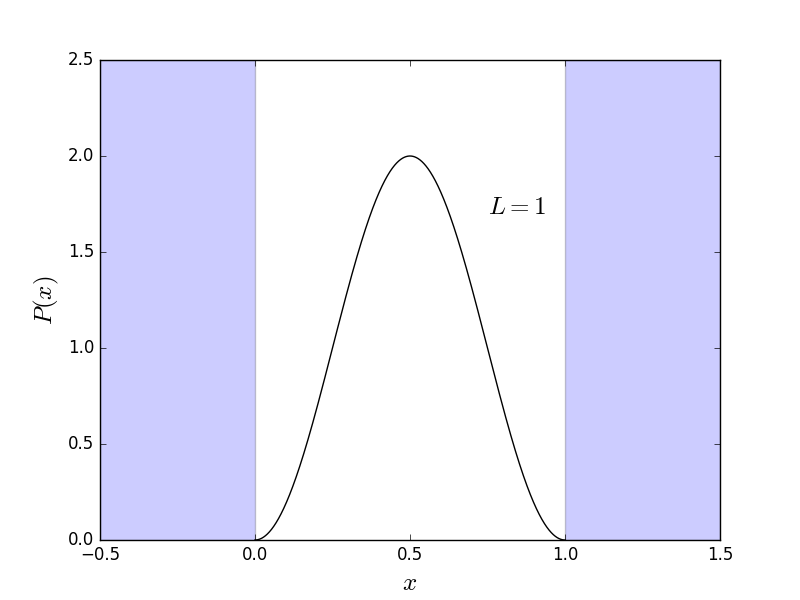
\includegraphics[scale=.28]{figure_4_isw}}}%
\caption{The radial probability distribution for the ground state of hydrogen. The radius of highest probability corresponds to the bohr radius $a_{0}$, which is set to 1 here. Also
shown is the positional probability distribution of the infinite square well of length $L = 1$.}
\end{figure}

Now, when we bring the two hydrogen atoms close to one another, the well width doubles and the individual wave functions overlap as shown in Figure 5 (TO DO: finish potential well explanation.). \par

Our goal now is to establish a description of the covalently bonded system through the use of a linear combination of ground state orbitals. Let $\ket{\psi_{0,1}}$ and $\ket{\psi_{0,2}}$
be the ground states of the first and second hydrogen atom, respectively. Then, $\ket{\psi_{0,1}}$ and $\ket{\psi_{0,2}}$ are clearly solutions to the Schroedinger equations
$$H\ket{\psi_{0,1}} = (K + V_{1})\ket{\psi_{0,1}} = E_{0}\ket{\psi_{0,1}} $$
$$H\ket{\psi_{0,2}} = (K + V_{2})\ket{\psi_{0,2}} = E_{0}\ket{\psi_{0,2}}$$
where $K$ is the kinetic energy of the electron, and $V_{i}$ is the nuclear potential from site $i$. We will describe the ground state of a single electron orbiting the two hydrogen neighbors as a linear combination of these individual ground states. That is,
$$ \ket{\psi_{0}} = c_{1}\ket{\psi_{0,1}} + c_{2}\ket{\psi_{0,1}}  $$
We can roughly approximate $\ket{\psi_{0,1}}$ and $\ket{\psi_{0,2}}$ to be orthogonal. As shown in Figure 5 (TO BE ADDED), the individual ground states are localized to either side of the potential well and
there is little overlap between the states given that the internucleic distance is not too short. This approximation allows us to establish the following orthogonality condition.
$$ \bra{\psi_{0,i}}\ket{\psi_{0,j}} = \delta_{ij}$$.
Now we will attempt to solve the Schroedinger equation to find the new ground state energy of the bonded system. The Schroedinger Equation is simply
$$H\ket{\psi_{0}} = E\ket{\psi_{0}}$$
We have not yet established the form of the Hamiltonian, but we can make two observations. The first is that the Hamiltonian can be written as the sum of the kinetic energy of the electron, as well as the potential energy contributions from each
of the hydreogen nuclei. That is,
$$ H = K + V_{1} + V_{2}$$
The second observation is that the Schroedinger equation can be written in a more explicit form. In this case, the new bonding ground state is a linear combination of two ground state orbitals - therefore, the
Hamiltonian is a $2\times 2$ matrix.
$$ \begin{bmatrix} H_{11} & H_{12}\\ H_{21}&H_{22} \end{bmatrix}\begin{bmatrix} c_{1} \\ c_{2} \end{bmatrix} = E\begin{bmatrix} c_{1} \\ c_{2} \end{bmatrix}$$
This yields the following system of equations
$$\sum_{j}H_{ij}c_{j} = Ea_{i}$$
where
$$H_{ij} = \bra{\psi_{0,i}}H\ket{\psi_{0,j}} = \bra{\psi_{0,i}}K + V_{1} + V_{2}\ket{\psi_{0,j}}$$
This allows us to examine the components of the Hamiltonian matrix.
$$H_{11} = \bra{\psi_{0,1}}K + V_{1}\ket{\psi_{0,1}} + \bra{\psi_{0,1}}V_{2}\ket{\psi_{0,1}} = E_{0} + V_{cross}$$
$$H_{22} = \bra{\psi_{0,2}}K + V_{2}\ket{\psi_{0,2}} + \bra{\psi_{0,2}}V_{1}\ket{\psi_{0,2}} = E_{0} + V_{cross}$$
$$H_{12} = \bra{\psi_{0,1}}K + V_{2}\ket{\psi_{0,2}} + \bra{\psi_{0,1}}V_{1}\ket{\psi_{0,2}} = -t$$
$$H_{21} = \bra{\psi_{0,2}}K + V_{2}\ket{\psi_{0,1}} + \bra{\psi_{0,2}}V_{1}\ket{\psi_{0,1}} = -t^{*}$$
where we have defined $V_{cross} = \bra{\psi_{0,2}}V_{1}\ket{\psi_{0,2}} = \bra{\psi_{0,1}}V_{2}\ket{\psi_{0,1}}$ and the \emph{hopping} term $ -t = \bra{\psi_{0,1}}V_{1}\ket{\psi_{0,2}}$. The $V_{cross}$ term represents the Coulomb potential
due to neighboring sites (i.e. the \emph{other} hydrogen nucleus). The hopping element $t$ represents the mechanism by which the electron can move from one orbital to another. To obtain the eigenenergies, we can diagonalize this Hamiltonian as follows.
$$det(H - EI) = \begin{vmatrix} E_{0} + V_{cross} - E & -t \\ -t^{*} & E_{0} + V_{cross} - E\end{vmatrix} = 0$$
From which we obtain
$$  (E_{0} + V_{cross} - E)^{2} - |t|^{2} = 0$$
$$ E^{2} - 2E(E_{0} + V_{cross}) + (E_{0} + V_{cross})^{2} - |t|^{2} = 0$$
Using the quadratic equation, we obtain the solution
$$E_{\pm} = E_{0} + V_{cross} \pm |t|$$
Now, we will find the eigenstates associated with the new ground state energies. The Schroedinger equation, again, is
$$ \begin{bmatrix} E_{0} + V_{cross} & -t\\ -t^{*} & E_{0} + V_{cross} \end{bmatrix}\begin{bmatrix} c_{1} \\ c_{2} \end{bmatrix} = E_{\pm}\begin{bmatrix} a_{1} \\ a_{2} \end{bmatrix}$$
which gives us the following system of equations to solve for $c_{1}$ and $c_{2}$
$$ (E_{0} + V_{cross})c_{1} -tc_{2} = E_{\pm}c_{1} $$
$$ (E_{0} + V_{cross})c_{2} -t*c_{1} = E_{\pm}c_{2} $$
Our associated normalized eigenvectors are therefore
$$\ket{\psi_{+}} = \frac{1}{\sqrt{2}}\ket{\psi_{0,1}} - \frac{1}{\sqrt{2}}\ket{\psi_{0,2}}$$
$$\ket{\psi_{-}} = \frac{1}{\sqrt{2}}\ket{\psi_{0,1}} + \frac{1}{\sqrt{2}}\ket{\psi_{0,2}}$$
The first thing to notice here is that while the individual hydrogen atoms have a single ground state orbital, when the atoms are brought close together, the delocalized ground state orbital actually splits into two levels.
The lower energy level (with energy $E_{-}$) is called the \emph{bonding} orbital because it promotes bonding by lowering the ground state energy. The higher energy orbital (associated with $E_{+}$) is called the \emph{antibonding} orbital. This is somewhat easier to understand
if we factor in Coulomb repulsion between the neighboring nuclei and allow the $V_{cross}$ term to vanish. In that case, we have
$$ E_{\pm} = E_{0} \pm |t| $$
So clearly, the bonding orbital has an energy lower than the original ground state energy and the antibonding orbital is associated with an energy higher than the original ground state energy. It is also worth noting that the difference between the bonding and antibonding energy levels is
proportional to the hopping term. In the limit that the hopping term vanishes, indicating that there is no possibility to hop between sites, the ground state energies converge back to the original ground state energy of hydrogen.

\subsection{Next Steps: One Dimensional Chain of Atomic Sites}
We will now generalize our model a bit by considering a one-dimensional chaing of $N$ sites, as opposed to two. First, we establish some properties of
our chain:
\begin{itemize}
\item There is a single orbital on each atomic site -  we will denote the orbital on site $i$ as $\ket{i}$.
\item Periodic boundary conditions are enforced. That is, site $N+1$ is site $1$.
\item Orbitals are taken to be orthogonal to one another. Therefore, $\bra{i}\ket{j} = \delta_{ij}$.
\item The interatomic spacing - distance between sites - is denoted $a$.
\end{itemize}

\begin{figure}[h]
\centering
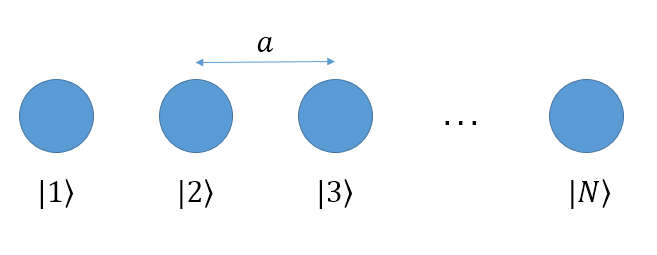
\includegraphics[scale=.5]{figure_6}
\caption{One dimensional chain of atomic sites. There is a single orbital at each site, denoted by $\ket{i}$. Interatomic spacing is $a$.}
\end{figure}

As before, we will consider a single electron moving around the chain of sites. The wavefunction for the electron is a linear combination of the atomic orbitals.
$$\ket{\psi} = \sum_{n = 1}^{N} = c_{n}\ket{n}$$
As before, we will use the Schroedinger equation to establish the eigenenergies and eigenstates of the system.
$$H\ket{\psi} = E\ket{\psi}$$
We observe the following about the Hamiltonian $H$:
$$ H = K + \sum_{j} V_{j} $$
$$ H_{nm} = \bra{n}H\ket{m} $$
where, as before, $K$ is the kinetic energy of the electron and $V_{j}$ is the Coulomb interaction due to site $j$. We can derive the elements of the
Hamiltonian matrix, $H_{nm}$, as follows:
$$ H\ket{m} = (K + \sum_{j}V_{j})\ket{m} $$
$$ = (K + V_{m})\ket{m} + \sum_{j \neq m}V_{j}\ket{m}$$
$$ = E_{0}\ket{m} + \sum_{j \neq m}V_{j}\ket{m} $$
where $E_{0}$ here is meant to be the energy associated with the orbital on a single atomic site. Therefore,
$$ \bra{n}H\ket{m} = E_{0}\bra{n}\ket{m} + \sum_{j \neq m}\bra{n}V_{j}\ket{m}$$
$$ = \delta_{nm} + \sum_{j \neq m}\bra{n}V_{j}\ket{m}$$
The last term can be summarized in the following way:
$$ \sum_{j \neq m}\bra{n}V_{j}\ket{m} = \left\{\begin{matrix}
                                                  V_{0}  &  n = m\\
                                                  -t  &  n = m \pm 1\\
                                                  0  & otherwise
                                                    \end{matrix}\right.$$
The idea is the following:
\begin{itemize}
\item In the case $n = m$, $V_{0}$ represents a sum of all $V_{cross}$ terms over the lattice. That is, it is the shift in the
      site energy due to Coulomb interactions with other sites.
\item When $n = m \pm 1$, then $\ket{n}$ and $\ket{m}$ are nearest neighbors. In that case, $\bra{n}V_{n}\ket{m}$ is defined to be $-t$,
the hopping term that takes the electron from site $m$ to site $n$. All other contributions in the sum vanish -- that is, we only consider
nearest neighbor hopping (right?).

\end{itemize}
Therefore, the elements of the Hamiltonian are given by
$$ \bra{n}H\ket{m} = (E_{0} + V_{0})\delta_{nm} - t(\delta_{n+1,m} + \delta_{n-1,m}) $$
The Ansatz solution for the eigenstate is given (in component form) as:
$$ c_{n} = \frac{e^{-ikna}}{\sqrt{N}} $$
where $c_{n}$ is the probability amplitude of the state $\ket{n}$, $k$ is the wavevector of the electron, and the $1/\sqrt{N}$ term normalizes the wavefunction. TODO: Periodicity and boundary conditions.
The periodicity of the solution can be examined by observing that $e^{-i2n\pi} = 1$ for arbitrary integer $n$ and writing
$$ c_{n} = \frac{e^{-ikna}}{\sqrt{N}} = \frac{e^{-ikna}}{\sqrt{N}}e^{-i2n\pi} $$
$$ = \frac{e^{-i(kna + 2n\pi)}}{\sqrt{N}} = \frac{e^{-i(k + 2\pi/a)na}}{\sqrt{N}}$$
Therefore the solution for $k$ is identical to the solution for $k + 2\pi/a$. When we enforce the periodic boundary conditions that site $n = 1$ is equivalent to site $n = N+1$, we find that $k$ is quantized
in units of $2\pi/Na$. Explicitly,
$$c_{1} = c_{N+1}$$
$$ \frac{e^{-ika}}{\sqrt{N}} = \frac{e^{-ik(N+1)a}}{\sqrt{N}}$$
$$ 1 = e^{-ikNa} $$
The above equation can only be true if $k$ is an integer multiple of $2\pi/Na$. \par
Now, if we plug our ansatz into the system of equations produced by the Schroeding equation,
$$ \sum_{m}H_{nm}c_{m} = Ec_{n}$$
$$ \sum_{m}H_{nm}\frac{e^{-ikma}}{\sqrt{N}} = E\frac{e^{-ikna}}{\sqrt{N}}$$
$$ \sum_{m}[(E_{0} + V_{0})\delta_{nm} - t(\delta_{n+1,m} + \delta_{n-1,m})]\frac{e^{-ikma}}{\sqrt{N}} = E\frac{e^{-ikna}}{\sqrt{N}}$$
$$ (E_{0} + V_{0})\frac{e^{-ikna}}{\sqrt{N}} - t\left (\frac{e^{-ik(n+1)a}}{\sqrt{N}} + \frac{e^{-ik(n-1)a}}{\sqrt{N}}\right ) = E\frac{e^{-ikna}}{\sqrt{N}}$$
$$  (E_{0} + V_{0})\frac{e^{-ikna}}{\sqrt{N}} - t\frac{e^{-ikna}}{\sqrt{N}}2cos(ka) = E\frac{e^{-ikna}}{\sqrt{N}} $$
$$ (E_{0} + V_{0}) - t2cos(ka) = E$$
The last equation is our dispersion relation $E(k)$, which describes the range of allowed energies for an electron floating through the lattice. The dispersion relation is plotted in Figure 7.
\begin{figure}[h]
\centering
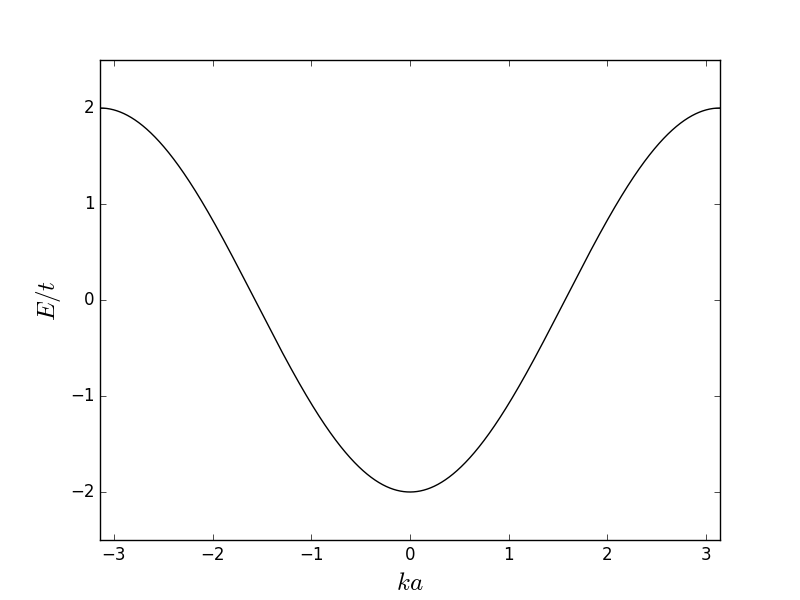
\includegraphics[scale=.5]{dispersion_1d}
\caption{Dispersion relation for one-dimensional monoatomic chain with interatomic distance $a$. Dispersion relation is plotted in units of $t$, as a function of $ka$, allowing $(E_{0} + V_{0})$ to vanish.}
\end{figure}
There are a few observations we can make from the plot of the dispersion relation. The first is that the width of the allowed energies is a function of the hopping element $t$. There is at least one $k$-state that has an energy in this band. The allowed
values for $ka$ are functions of $N$ such that
$$ ka = \frac{2\pi}{N}m $$
where m is some integer. Therefore, when N = 1 (the one site limit), $k$ can only take on values $0$, $2\pi$, $4\pi$, etc. - all of which map to the same energy so only a single energy is allowed. As N grows, we increase the number of allowed $ka$ values
within a $2\pi$ range and, therefore, increase the number of discrete energy levels until the band is saturated in the $N \rightarrow \infty$ limit.


\subsection{Arbitrary Crystal Structure}
Now, we shift our focus to applying the tight binding model to an arbitrary crystal structure with multiple orbitals per site. Our discussion will closely follow that found in \cite{mccann}. In the general case, we have
$N$ identical atomics sites with $M$ orbitals per site. For each of the $M$ orbitals, we can write down a Bloch state which represents the wavefunction of the electron in the periodically repeating lattice.

$$ \Phi_m = \frac{1}{\sqrt{N}}\sum_{n = 1}^{N}e^{i\vec{k}\cdot\vec{R}_{m,n}}\phi_{m}{\vec{r} - \vec{R}_{m,n}} $$

where $\phi_{m}$ is the $m$th orbital and $\vec{R}_{m,n}$ is the corresponding position of this orbital on the $n$th site. We should notice that these Bloch states are simply generalizations of the one-dimensional, single
orbital solution. The full electronic wave function is a sum over the $M$ bloch states and is given by
$$ \psi = \sum_{m = 1}^{M}c_{m}\Phi_m$$
where $c_m$ are the coefficients of linear superposition. To determine these coefficients, we can plug our expression for $\psi$ into the Schroedinger equation.
\subsubsection{One dimensional chain of atomic sites revisited}
To see the effect of multiple orbitals per site, we will consider an extension of the one-dimensional chain where each atomic site has two orbitals. TODO: Finish section.


\section{Monolayer Graphene}
We now use the tight binding model to analyze the band structure of a single layer of graphene. Graphene can be thought of as a lattice where each site contains the unit cell shown in Figure 8. That is, each site in
the lattice contains two carbon atoms, which we will label $A$ and $B$.


\begin{figure}[h]
\centering
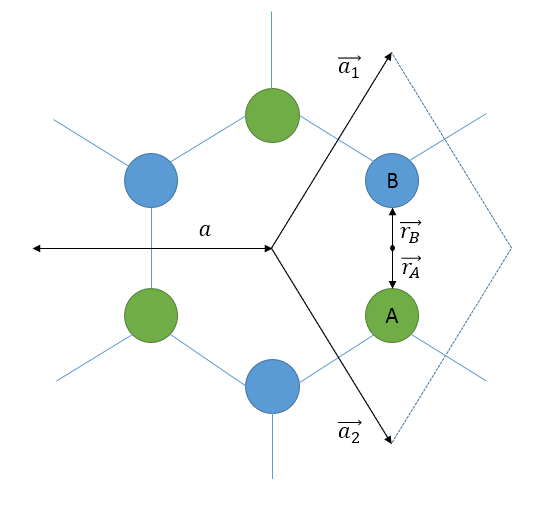
\includegraphics[scale=.5]{monolayer}
\caption{Diagram of hexagonal lattice structure of monolayer graphene. The unit cell is outlined with a dashed line, containing two carbon atoms labeled $A$ and $B$. denoted by $\ket{i}$. The width of the honeycomb is $a$, which
yields two primitive lattice vectors $\vec{a}_{1} = (\frac{a}{2}, \frac{\sqrt{3}a}{2})$ and $\vec{a}_{2} = (\frac{a}{2}, -\frac{\sqrt{3}a}{2})$.}
\end{figure}

From each carbon atom, we only consider a single $2p_{z}$ orbital. As described in the first section, the remaining valence electrons are tied
up in $\sigma$ bonds via $sp^{2}$ hybridization. Let's begin by writing down the very general electronic wavefunction.
$$\psi_{k} = \sum_{m = 1}^{M} c_{m}\Phi_{m}$$
where $\Phi_{m}$ is the Bloch state defined by
$$\Phi_{m} = \frac{1}{\sqrt{N}}\sum_{n=1}^{N} e^{i\vec{k}\cdot\vec{R}_{n}}\phi_{m}(\vec{r} - \vec{R}_{n})$$
The vector $\vec{R}_{n}$ represents the position of the $n$th unit cell over a total of $N$ unit cells. In our case, the index $m$ will only sum over the sites $A$ and $B$ within the unit cell.
Therefore, in the case of monolayer graphene, we can explicitly write
$$ \psi_{k} = \frac{1}{\sqrt{N}}(c_{A}\sum_{n}e^{i\vec{k}\cdot\vec{R}_{n}}\phi_{A} + c_{B}\sum_{n}e^{i\vec{k}\cdot\vec{R}_{n}}\phi_{B}) $$
where $\phi_{A}$ and $\phi_{B}$ are the $2p_{z}$ wavefunctions for sites $A$ and $B$, respectively. The Hamiltonian is directly analogous to the one-dimensional chain example:
$$ H = K + \sum_{n}V_{A} + V_{B} $$
where
$$V_{A} = V(\vec{r} - \vec{r}_{A} - \vec{R}_n)$$
$$V_{B} = V(\vec{r} - \vec{r}_{B} - \vec{R}_n)$$
If we apply the Hamiltonian to the $\phi_{A}$ orbital, for example, we obtain the following:
$$H\phi_{A} = (K + \sum_{n}V_{A} + V_{B})\phi_{A}$$
$$ = E_{A} + [(\sum_{n, \vec{R}_{n} \neq 0}V_{A} + V_{B}) + V(\vec{r} - \vec{r}_{B})] \phi_{A}$$
where $E_{A} = E_{B}$ is the energy of $2p_{z}$ orbital. We will simplify a bit by allowing $E_{A} = E_{B} = 0$. Therefore, we obtain the two equations
$$H\phi_{A,B} = [(\sum_{n, \vec{R}_{n} \neq 0}V_{A} + V_{B}) + V(\vec{r} - \vec{r}_{B,A})] \phi_{A,B} = \Delta U_{A,B}\phi_{A,B}$$
where we have defined $\Delta U$ as the potential energy term of the Hamiltonian. \par
Now, we will apply the Hamiltonian to the electronic wavefunction $\psi_{k}$:
$$H\psi_{k} = E(\vec{k})\psi_{k}$$
From here, it is easy to see
$$\bra{\phi_{A,B}}H\ket{\psi_{k}} = \bra{\phi_{A,B}}E(\vec{k})\ket{\psi_{k}}$$
From which we obtain
$$E(\vec{k}) = \frac{\bra{\phi_{A,B}}\Delta U_{A,B}\ket{\psi_{k}}}{\bra{\phi_{A,B}}\ket{\psi_{k}}}$$
We begin by calculating the denominator terms. In the following, we take only nearest neighbor overlap terms into account. That is,
$$\sum_{n}e^{i\vec{k}\cdot\vec{R}_{n}}\bra{\phi_{A}}\ket{\phi_{A}} = \bra{\phi_{A}}\ket{\phi_{A}} = 1$$
$$\sum_{n}e^{i\vec{k}\cdot\vec{R}_{n}}\bra{\phi_{A}}\ket{\phi_{B}}) = \bra{\phi_{A}}\ket{\phi_{B}}(1 + e^{i\vec{k}\cdot-\vec{a}_{1}} + e^{i\vec{k}\cdot\vec{a}_{2}})$$
Now, we get, dropping the normalization factor,
$$\bra{\phi_{A}}\ket{\psi_{k}} = c_{A} + c_{B}\bra{\phi_{A}}\ket{\phi_{B}}(1 + e^{i\vec{k}\cdot-\vec{a}_{1}} + e^{i\vec{k}\cdot\vec{a}_{2}}) $$
$$\bra{\phi_{B}}\ket{\psi_{k}} = c_{B} + c_{A}\bra{\phi_{B}}\ket{\phi_{A}}(1 + e^{i\vec{k}\cdot\vec{a}_{1}} + e^{i\vec{k}\cdot-\vec{a}_{2}})$$

Evaluating the numerator gives us
$$\bra{\phi_{A}}\Delta U_{A}\ket{\psi_{k}} = c_{B}\bra{\phi_{A}}\Delta U_{A}\ket{\phi_{B}}(1 + e^{i\vec{k}\cdot-\vec{a}_{1}} + e^{i\vec{k}\cdot\vec{a}_{2}})$$
$$\bra{\phi_{B}}\Delta U_{B}\ket{\psi_{k}} = c_{A}\bra{\phi_{B}}\Delta U_{B}\ket{\phi_{A}}(1 + e^{i\vec{k}\cdot\vec{a}_{1}} + e^{i\vec{k}\cdot-\vec{a}_{2}})$$

Now, we'll simplify things by introducing some shorthand notation. Let
$$ \alpha =  1 + e^{i\vec{k}\cdot-\vec{a}_{1}} + e^{i\vec{k}\cdot\vec{a}_{2}}$$
$$ \gamma_{0} = \bra{\phi_{A}}\ket{\phi_{B}} = \bra{\phi_{B}}\ket{\phi_{A}}$$
$$ \gamma_{1} = \bra{\phi_{A}}\Delta U_{A}\ket{\phi_{B}} = \bra{\phi_{B}}\Delta U_{B}\ket{\phi_{B}}$$

To remind ourselves, our equation for $E(\vec{k})$ is
$$E(\vec{k}) = \frac{\bra{\phi_{A,B}}\Delta U_{A,B}\ket{\psi_{k}}}{\bra{\phi_{A,B}}\ket{\psi_{k}}}$$
and with the values we've calculated, we obtain the following system of equations:
$$E(\vec{k})(c_{A} + \alpha\gamma_{0}c_{B}) = \alpha\gamma_{1}c_{B}$$
$$E(\vec{k})(c_{B} + \alpha^{*}\gamma_{0}c_{A}) = \alpha^{*}\gamma_{1}c_{A}$$
So, the eigenvalue equation is given by

$$
\begin{bmatrix}
E(\vec{k}) & \alpha\gamma_{0}E(\vec{k}) - \alpha\gamma_{1}\\
  \alpha^{*}\gamma_{0}E(\vec{k}) - \alpha^{*}\gamma_{1} & E(\vec{k})
\end{bmatrix}
\begin{bmatrix}
c_{A} \\
c_{B}
\end{bmatrix}
= 0
$$
Taking the determinant gives us the characteristic equation
$$E(\vec{k})^{2}(1 - |\alpha|^2\gamma_{0}^{2}) + 2|\alpha|^2\gamma_{0}\gamma_{1}E(\vec{k}) - |\alpha|^2\gamma_{1}^{2} = 0$$
Now, if we make the assumption (as we've done in previous sections) that the orbital overlap is so small that they are practically orthogonal,
we end up with
$$\bra{\phi_{B}}\ket{\phi_{A}} = \bra{\phi_{1}}\ket{\phi_{B}} = \gamma_{0} = 0$$
which allows us to obtain the following simple equation for the energy $E(\vec{k})$:
$$ E(\vec{k}) = \pm |\alpha|\gamma_{1}$$
To obtain an explicit expression for $E(\vec{k})$, we begin by calculating the magnitude of $\alpha$. First, we note the following form for $\alpha$:
$$\alpha = 1 + e^{i\vec{k}\cdot-\vec{a}_{1}} + e^{i\vec{k}\cdot\vec{a}_{2}}$$
$$= 1 + exp\left (-i\left (k_{x}\frac{a}{\sqrt{2}} + k_{y}\frac{3a}{\sqrt{2}}\right )\right ) + exp\left (i\left (k_{x}\frac{a}{\sqrt{2}} - k_{y}\frac{3a}{\sqrt{2}}\right )\right )$$
$$ = 1 + exp\left (-ik_{y}\frac{3a}{\sqrt{2}}\right )\left (exp\left (-ik_{x}\frac{a}{\sqrt{2}}\right ) + exp\left (ik_{x}\frac{a}{\sqrt{2}}\right )\right )$$
$$ = 1 + exp\left (-ik_{y}\frac{3a}{\sqrt{2}}\right )\left ( 2cos\left (k_{x}\frac{a}{\sqrt{2}}\right )\right )$$
Using this form, we now calculate the magnitude of $\alpha$.
$$|\alpha| = \sqrt{\alpha^{*}\alpha}$$
$$= \sqrt{\left [1 + exp\left (-ik_{y}\frac{3a}{\sqrt{2}}\right )\left ( 2cos\left (k_{x}\frac{a}{\sqrt{2}}\right )\right )\right ]
          \left [1 + exp\left (+ik_{y}\frac{3a}{\sqrt{2}}\right )\left ( 2cos\left (k_{x}\frac{a}{\sqrt{2}}\right )\right )\right ]}$$
$$ = \sqrt{1 + 4cos\left ( k_{y}\frac{3a}{\sqrt{2}}\right )cos\left ( k_{y}\frac{a}{\sqrt{2}}\right ) + 4cos^{2}\left (k_{x}\frac{a}{\sqrt{2}}\right ) }$$
Finally, we obtain the final equation for the dispersion relation of monolayer graphene.
$$ E(\vec{k}) = \pm \gamma_{1}\sqrt{1 + 4cos\left ( k_{y}\frac{3a}{\sqrt{2}}\right )cos\left ( k_{y}\frac{a}{\sqrt{2}}\right ) + 4cos^{2}\left (k_{x}\frac{a}{\sqrt{2}}\right ) }$$
The dispersion relation is plotted in figure 8.
\begin{figure}[h]
\centering
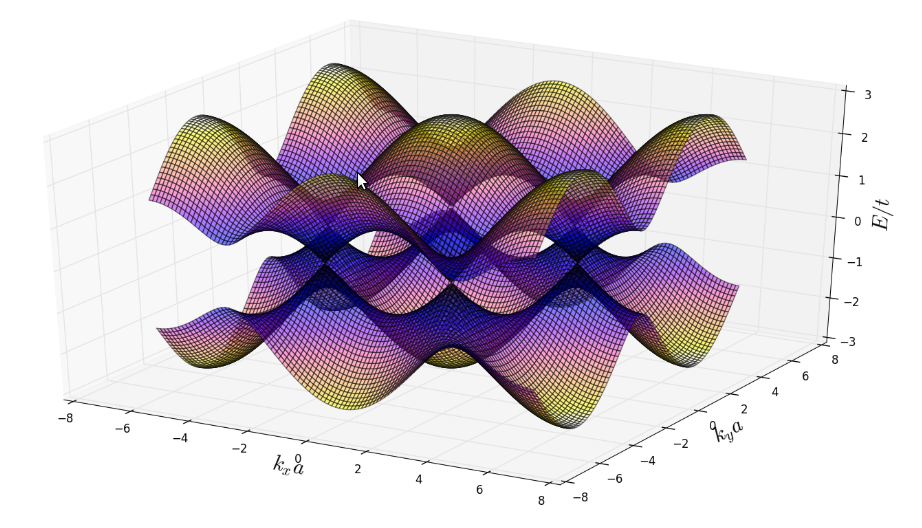
\includegraphics[scale=.42]{monolayer_disp_small}
\caption{Dispersion relation $E(\vec{k})$ plotted for monolayer graphene. }
\end{figure}
\section{Bilayer Graphene}
Finally, we take a look at the bilayer case. When considering two layers of graphene, our unit cell grows by two sites. That is, we not only consider the
two carbon atoms in the unit cell of the bottom lattice as well as two carbon atoms in the unit cell of the top lattice. Within the bilayer unit cell,
we have four sites: $A_{1}$ and $B_{1}$ on the bottom layer, and $A_{2}$ and $B_{2}$ on the top layer. The layers are stacked such that $A_{2}$ lies
directly on top of $B_{1}$, but $A_{1}$ and $B_{2}$ are not aligned. For this reason, $A_{2}$ and $B_{1}$ are referred to as "dimer" sites while
$A_{1}$ and $B_{2}$ are non-dimer sites. The configuration of the unit cell is shown in figure 9. \par
\begin{figure}[h]
\centering
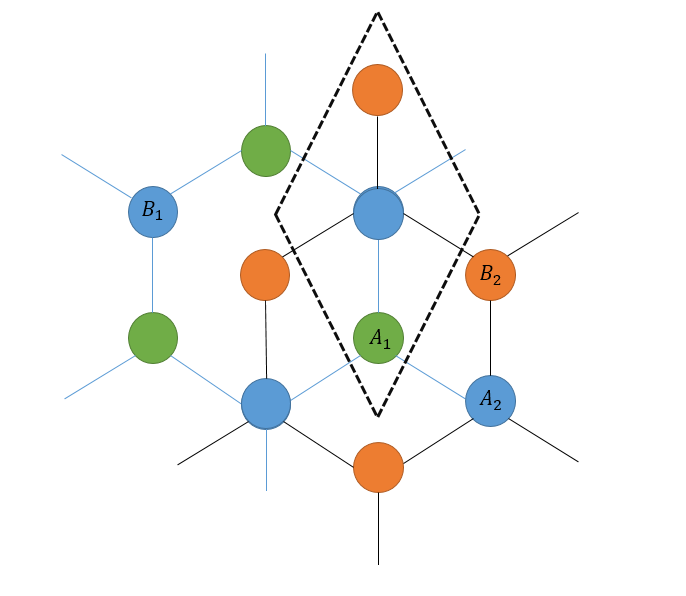
\includegraphics[scale=.50]{bilayer}
\caption{The top layer, containg $A_{2}$ and $B_{2}$, is shown with blue and orange sites. The bottom layer, containing $A_{1}$ and $B_{1}$, is shown with green and blue sites.
The sites $A_{2}$ and $B_{1}$ are both colored blue to indicate dimer sites. The unit cell is bounded by the dashed lines. }
\end{figure}
\begin{figure}[h]
\centering
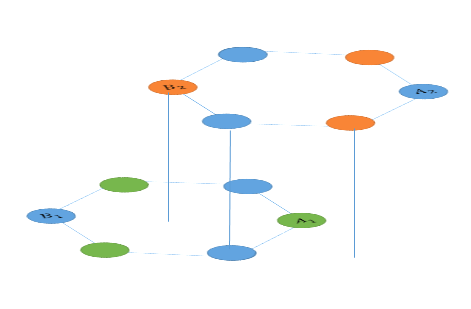
\includegraphics[scale=.62]{bilayer2}
\caption{A side view of the configuration of bilayer graphene. }
\end{figure}
We begin by formalizing the techniques of the last section and observing that the energy $E(\vec{k})$ satisfies the following relation:
$$H\psi_{k}=E(\vec{k})S\psi_{k}$$
where $\psi_{k}$ is the electronic wavefunction, $H$ is the \emph{transfer integral matrix} and $S$ is the \emph{overlap integral matrix}. The
matrices are defined by
$$H_{ij} = \bra{\Phi_{i}}\mathcal{H}\ket{\Phi_{j}}$$
and
$$S_{ij} = \bra{\Phi_{i}}\ket{\Phi_{j}}$$
where $\mathcal{H}$ is the Hamiltonian and $\Phi_{i}$ is the Bloch state corresponding to orbital $i$, where $i$ takes on the values $A_{1}$, $B_{1}$, $A_{2}$, and $B_{2}$. Now, the Hamiltonian $\mathcal{H}$
is given by
$$ \mathcal{H} = K + \sum_{n}V_{A_{1}} + V_{B_{1}} + V_{A_{2}} + V_{B_{2}} $$
where
$$V_{i} = V(\vec{r} - \vec{r}_{i} - \vec{R}_n)$$
which is analogous to what we see in the monolayer case. First, let's consider the overlap integral matrix $S$. The on-diagonal elements are
given by
$$S_{mm} = \bra{\Phi_{m}}\ket{\Phi_{m}}$$
$$ = \frac{1}{N} \sum_{n'=1}^{N} e^{-i\vec{k}\cdot\vec{R}_{n'}} \sum_{n=1}^{N} e^{i\vec{k}\cdot\vec{R}_{n}} \bra{\phi_{m}(\vec{r} - \vec{R}_{n'})}\ket{\phi_{m}(\vec{r} - \vec{R}_{n})} $$
As before, we will only consider nearest neighbor contributions. Therefore, there is no overlap between a particular orbital and its corresponding orbital
in another unit cell. We only consider the case where $R_{n'} = R_{n}$. This simplifies to
$$S_{mm} = \frac{1}{N}\sum_{n}^{N}\bra{\phi_{m}(\vec{r} - \vec{R}_{n})}\ket{\phi_{m}(\vec{r} - \vec{R}_{n})} = 1$$
Now, the off-diagonal elements are given by
$$ S_{m'm} = \frac{1}{N} \sum_{n'=1}^{N} e^{-i\vec{k}\cdot\vec{R}_{n'}} \sum_{n=1}^{N} e^{i\vec{k}\cdot\vec{R}_{n'}} \bra{\phi_{m'}(\vec{r} - \vec{R}_{n'})}\ket{\phi_{m}(\vec{r} - \vec{R}_{n})} $$
As with the monolayer case, we will consider nearest neighbor interations on the same layer, but we must also consider the interactions between the dimer sites $B_{1}$ and $A_{2}$. Since the nearest-neighbor
interactions are almost localized to the layer, the $S$ matrix will almost look block diagonal with two monolayer submatrices. However, we will also factor in the interlayer coupling. The nearest neighbor
interactions elements are given by:
$$ S_{A_{1}B_{1}} = S_{A_{2}B_{2}}= \alpha\gamma_{0}$$
$$ S_{B_{1}A_{1}} = S_{B_{2}A_{2}} = \alpha^{*}\gamma_{0} $$
which is directly analogous to the monolayer case. And for the dimer site coupling, we simply introduce the element $\gamma_{d}$.
Therefore, our $S$ matrix is given by
$$ S =
\begin{bmatrix}
1 & \alpha\gamma_{0} & 0 & 0\\
\alpha^{*}\gamma_{0} & 1 & \gamma_{d} & 0\\
0 & \gamma_{d} & 1 & \alpha\gamma_{0} \\
0 & 0 & \alpha^{*}\gamma_{0} & 1
\end{bmatrix}
$$

Now, let's consider the transfer integral matrix $H$. As with the overlap integral matrix, we can see that the monolayer subspace will be
the same as before. That is,
$$H_{A_{1,2}B_{1,2}} = -\alpha\gamma_{1}$$
$$H_{B_{1,2}A_{1,2}} = -\alpha^{*}\gamma_{1}$$
and
$$H_{A_{1,2}A_{1,2}} = E_{A_{1,2}}$$
$$H_{B_{1,2}A_{1,2}} = E_{B_{1,2}}$$

For the interlayer subspace, we introduce a number of parameters. First, we introduce $\beta_{d}$, an element to describe interlayer
coupling between dimer sites, which is strictly vertical.
$$ H_{A_{2}B_{1}} = H_{B_{1}A_{2}} = \beta_{d} $$

Then we introduce $\beta_{nd}$ and $\beta_{nn}$ for interactions between non-dimer/dimer pairs and non-dimer/non-dimer pairs respectively.
We must also consider the fact that these interlayer interactions are not strictly vertical and involve some component of in-plane
hopping. Therefore,
$$ H_{A_{2}B_{1}} = H_{B_{1}A_{2}} = \beta_{d} $$
$$ H_{A_{1}A_{2}} = H_{B_{1}B_{2}} = \alpha\beta_{nd} $$
$$ H_{A_{1}B_{2}} = -\alpha^{*}\beta_{nn} $$
$$ H_{A_{2}A_{1}} = H_{B_{2}B_{1}} = \alpha^{*}\beta_{nd} $$
$$ H_{B_{2}A_{1}} = -\alpha\beta_{nn} $$

where sign conventions are chosen for convenience. Putting this all together gives us:

$$ H =
\begin{bmatrix}
E_{A_{1}} & -\alpha\gamma_{1} & \alpha\beta_{nd} & -\alpha^{*}\beta_{nn}\\
-\alpha^{*}\gamma_{1} & E_{B_{1}} & \beta_{d} & \alpha\beta_{nd}\\
\alpha^{*}\beta_{nd} & \beta_{d} & E_{A_{2}} & -\alpha\gamma_{1} \\
-\alpha\beta_{nn} & \alpha^{*}\beta_{nd} & -\alpha^{*}\gamma_{1} & E_{B_{2}}
\end{bmatrix}
$$

Now, we need to solve the characteristic equation for $E(\vec{k})$.
\begin{equation}
det(H - E(\vec{k})S) = 0
\end{equation}
Using the table of experimentally realized values in Figure 11, and making the approximations
$\gamma_{0} = \gamma_{d} = 0$ and $E_{A_{1}} = E_{B_{1}} = E_{A_{2}} = E_{B_{2}} = 0$,  we obtain the
plot for the band structure of bilayer graphene presented in Figure 12.
\begin{figure}[h]

\centering
\begin{tabular}{ |c|c|c|  }
 \hline
 \multicolumn{3}{|c|}{Experimentally Realized Values for Bilayer Graphene} \\
 \hline
 Intralayer hopping   & $\gamma_{1}$   &  3.16 eV\\
 Dimer interlayer coupling & $\beta_{d}$ & .381 eV\\
 Non-dimer interlayer coupling & $\beta_{nn}$ & .38 eV\\
 Dimer/Non-dimer interlayer coupling & $\beta_{nd}$ & .14 eV\\
 \hline
\end{tabular}
\caption{Experimentally realized values used to plot $E(k)$. Values obtained from
\cite{mccann} and published in \cite{kuzmenko}.}
\end{figure}

\begin{figure}[h]
\centering
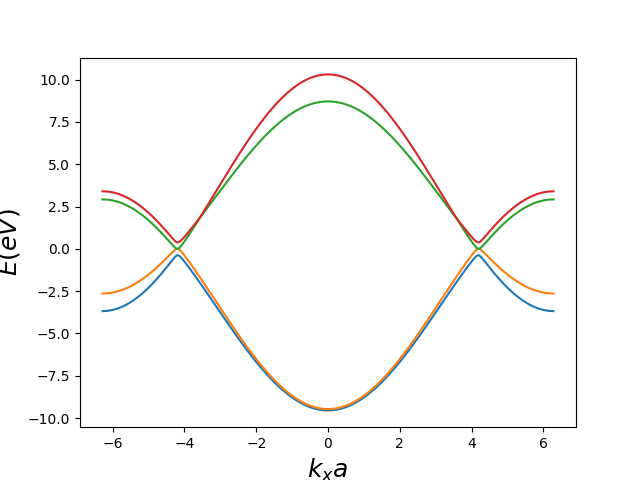
\includegraphics[scale=.62]{bilayer_band_3}
\caption{Band structure of bilayer graphene. $E_{k}$ is plotted along the $k_{x}a$ axis. }
\end{figure}

\begin{figure}[h]
\centering
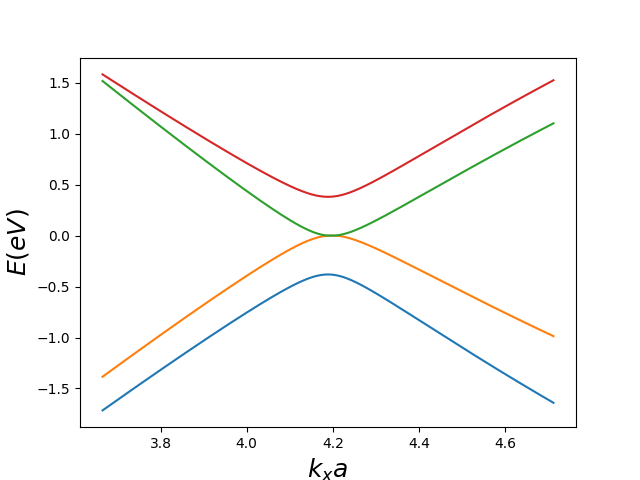
\includegraphics[scale=.62]{bilayer_band_kpos}
\caption{$E_{k}$ is plotted along the $k_{x}a$ axis. Plot is centered on the $K_{+}$ Dirac point at $k_{x} = \frac{4\pi}{3a}$. }
\end{figure}

\subsection{Low Energy Limit}
We can see from the energy dispersion plot in figure 12 that one conduction band and one valence band actually touch at the Dirac points $K_{+}$ and $K_{-}$.
To analyze the behavior around these points, we will look at the energy dispersion in the small region around the $K_{+}$ point. The $K_{+}$ point is located at
$(k_{x} = \frac{4\pi}{3a}, k_{y} = 0)$. TO DO: Insert figure for $K_{+}$ position derivation.
The $\vec{k}$-dependent element of our Hamiltonian is $\alpha$ (as well as, of course, $\alpha^{*}$). Let us first define
\begin{equation}
\vec{k}' = \vec{k} - K_{+}
\end{equation}
Then we have
\begin{equation}
\vec{k} = \vec{k}' + K_{+} = (k_{x}' + \frac{4\pi}{3a}, k_{y}')
\end{equation}
Therefore,
$$
\alpha = 1 + e^{i\vec{k}\cdot-\vec{a}_{1}} + e^{i\vec{k}\cdot\vec{a}_{2}}
$$
\begin{equation}
 = 1 + exp\left (-i\left (\frac{ak_{x}}{2} + \frac{\sqrt{3}ak_{y}}{2}\right )\right ) + exp\left (i\left (\frac{ak_{x}}{2} - \frac{\sqrt{3}ak_{y}}{2}\right )\right )
\end{equation}
\begin{equation}
 = 1 + exp\left (-i\left (\frac{ak_{x}'}{2} + \frac{2\pi}{3} + \frac{\sqrt{3}ak_{y}'}{2}\right )\right ) + exp\left (i\left (\frac{ak_{x}'}{2} + \frac{2\pi}{3} - \frac{\sqrt{3}ak_{y}'}{2}\right )\right )
\end{equation}
Now, we expand $\alpha(k_{x}', k_{y}')$ around the point $(k_{x}', k_{y}') = (0,0)$.
\begin{equation}
\alpha(k_{x}, k_{y}) = \alpha(0,0) + \alpha_{k_{x}}(0,0)k_{x} + \alpha_{k_{y}}(0,0)k_{y} + \mathcal{O}(k^{2})
\end{equation}
\begin{equation}
\alpha = -\frac{\sqrt{3}a}{2}(k_{x}' - ik_{y}')
\end{equation}
and similarly, we obtain
\begin{equation}
\alpha^{*} = -\frac{\sqrt{3}a}{2}(k_{x}' + ik_{y}')
\end{equation}
If we define $\kappa = k_{x}' - ik_{y}'$, then we can write
\begin{equation}
\alpha = -\frac{\sqrt{3}a}{2}\kappa
\end{equation}
and similarly, we obtain
\begin{equation}
\alpha^{*} = -\frac{\sqrt{3}a}{2}\kappa^{*}
\end{equation}
To remind ourselves, the Hamiltonian is given by
\begin{equation}
H =
\begin{bmatrix}
E_{A_{1}} & -\alpha\gamma_{1} & \alpha\beta_{nd} & -\alpha^{*}\beta_{nn}\\
-\alpha^{*}\gamma_{1} & E_{B_{1}} & \beta_{d} & \alpha\beta_{nd}\\
\alpha^{*}\beta_{nd} & \beta_{d} & E_{A_{2}} & -\alpha\gamma_{1} \\
-\alpha\beta_{nn} & \alpha^{*}\beta_{nd} & -\alpha^{*}\gamma_{1} & E_{B_{2}}
\end{bmatrix}
\end{equation}

The intralayer subspaces characterized by $\{A_{1}, B_{1}\}$ and $\{A_{2}, B_{2}\}$ simply take on the form
\begin{equation}
H_{mono} = \begin{bmatrix}
E_{A_{1,2}} & \frac{\sqrt{3}a}{2}\kappa\gamma_{1} \\
\frac{\sqrt{3}a}{2}\kappa^{*}\gamma_{1} & E_{B_{1,2}}
\end{bmatrix}
\end{equation}

which also characterizes the effect of expanding around the dirac points in the monolayer case. The full Hamiltonian is given by

\begin{equation}
H =
\begin{bmatrix}
E_{A_{1}} & \frac{\sqrt{3}a}{2}\kappa\gamma_{1} & -\frac{\sqrt{3}a}{2}\kappa\beta_{nd} & \frac{\sqrt{3}a}{2}\kappa^{*}\beta_{nn}\\
\frac{\sqrt{3}a}{2}\kappa^{*}\gamma_{1} & E_{B_{1}} & \beta_{d} & -\frac{\sqrt{3}a}{2}\kappa\beta_{nd}\\
-\frac{\sqrt{3}a}{2}\kappa^{*}\beta_{nd} & \beta_{d} & E_{A_{2}} & \frac{\sqrt{3}a}{2}\kappa\gamma_{1} \\
\frac{\sqrt{3}a}{2}\kappa\beta_{nn} & -\frac{\sqrt{3}a}{2}\kappa^{*}\beta_{nd} & \frac{\sqrt{3}a}{2}\kappa^{*}\gamma_{1}& E_{B_{2}}
\end{bmatrix}
\end{equation}

To obtain an analytic result for the energy eigenvalues, we will allow $E_{A_{1}{2}} = E_{B_{1,2}} = 0$ and we will also
allow $\beta_{nd}$ to vanish as the dimer/non-dimer coupling is the weakest of the coupling terms. This gives us

\begin{equation}
H =
\begin{bmatrix}
0 & \frac{\sqrt{3}a}{2}\kappa\gamma_{1} & 0 & \frac{\sqrt{3}a}{2}\kappa^{*}\beta_{nn}\\
\frac{\sqrt{3}a}{2}\kappa^{*}\gamma_{1} & 0 & \beta_{d} & 0 \\
0 & \beta_{d} & 0  & \frac{\sqrt{3}a}{2}\kappa\gamma_{1} \\
\frac{\sqrt{3}a}{2}\kappa\beta_{nn} & 0 & \frac{\sqrt{3}a}{2}\kappa^{*}\gamma_{1}& 0
\end{bmatrix}
\end{equation}

for which solving the characteristic eigenvalue equation yields the solutions

\begin{equation}
E = \pm \sqrt{\frac{\beta_d^{2}}{2} + a^{2}|\kappa|^{2}\left (\frac{3\gamma_{1}^{2}}{4} + \frac{3\beta_{nn}^{2}}{8}\right ) \pm \sqrt{\mathcal{O}(|\kappa|^{4})}}
\end{equation}

Furthermore, if we allow the $\beta_{nn}$ terms to vanish, the equation for the energy simply becomes
\begin{equation}
E = \pm\frac{1}{2}\left ( \beta_{d} \pm \sqrt{\beta_{d}^{2} + 3a^{2}|\kappa|^{2}\gamma_{1}^{2}} \right)
\end{equation}

In either case, the notable observation is that the dispersion relation is approximately linear with respect to $\kappa$ in the small regions around the Dirac points. That is, around the Dirac
points, the energy dispersion is approximately linear with the deviation in momentum space from the Dirac point. Furthermore, if we examine the simplified equation for energy at the
Dirac point itself (characterized by $|\kappa| = 0$), then we find the following allowed energies:
$$
E = 0
$$
\begin{equation}
E = \pm \beta_{d}
\end{equation}
The $E = 0$ energy corresponds to the bands that touch at the Dirac point. The $E = \pm \beta_{d}$ energies indicate a band gap
of size $2\beta_{d}$ between the higher energy conduction band and lower energy valence band.

% APPENDIX %
\section{Appendix}
\subsection{Nearest Neighbor Lattice Vectors}
To represent our position within the lattice, we have chosen the conventional lattice vector
\begin{equation}
\vec{R} = n_{1}\vec{a}_{1} + n_{2}\vec{a}_{2}
\end{equation}
where $\vec{a}_{1}$ and $\vec{a}_2$ are the primitive lattice vectors given by
$$\vec{a}_{1} = \left(\frac{a}{2}, \frac{\sqrt{3}a}{2}\right )$$
$$\vec{a}_{2} = \left(\frac{a}{2}, -\frac{\sqrt{3}a}{2}\right )$$
However, this choice is not unique and we could choose another system to represent our position within the lattice.
For example, instead of expressing our position in terms of $\vec{a}_{1}$ and $\vec{a}_{2}$, we might choose instead
to use the nearest neighbor distances $\vec{d}_{1}$, $\vec{d}_{2}$, $\vec{d}_{3}$ as diagrammed in Figure . Explicitly
written, these vectors are
$$ \vec{d}_{1} = \left(-\frac{a}{2}, \frac{a}{2\sqrt{3}}\right)$$
$$ \vec{d}_{2} = \left(\frac{a}{2}, \frac{a}{2\sqrt{3}}\right)$$
\begin{equation}
\vec{d}_{3} = \left (0, \frac{-2a}{\sqrt{3}}\right)
\end{equation}

\begin{figure}[h]
\centering
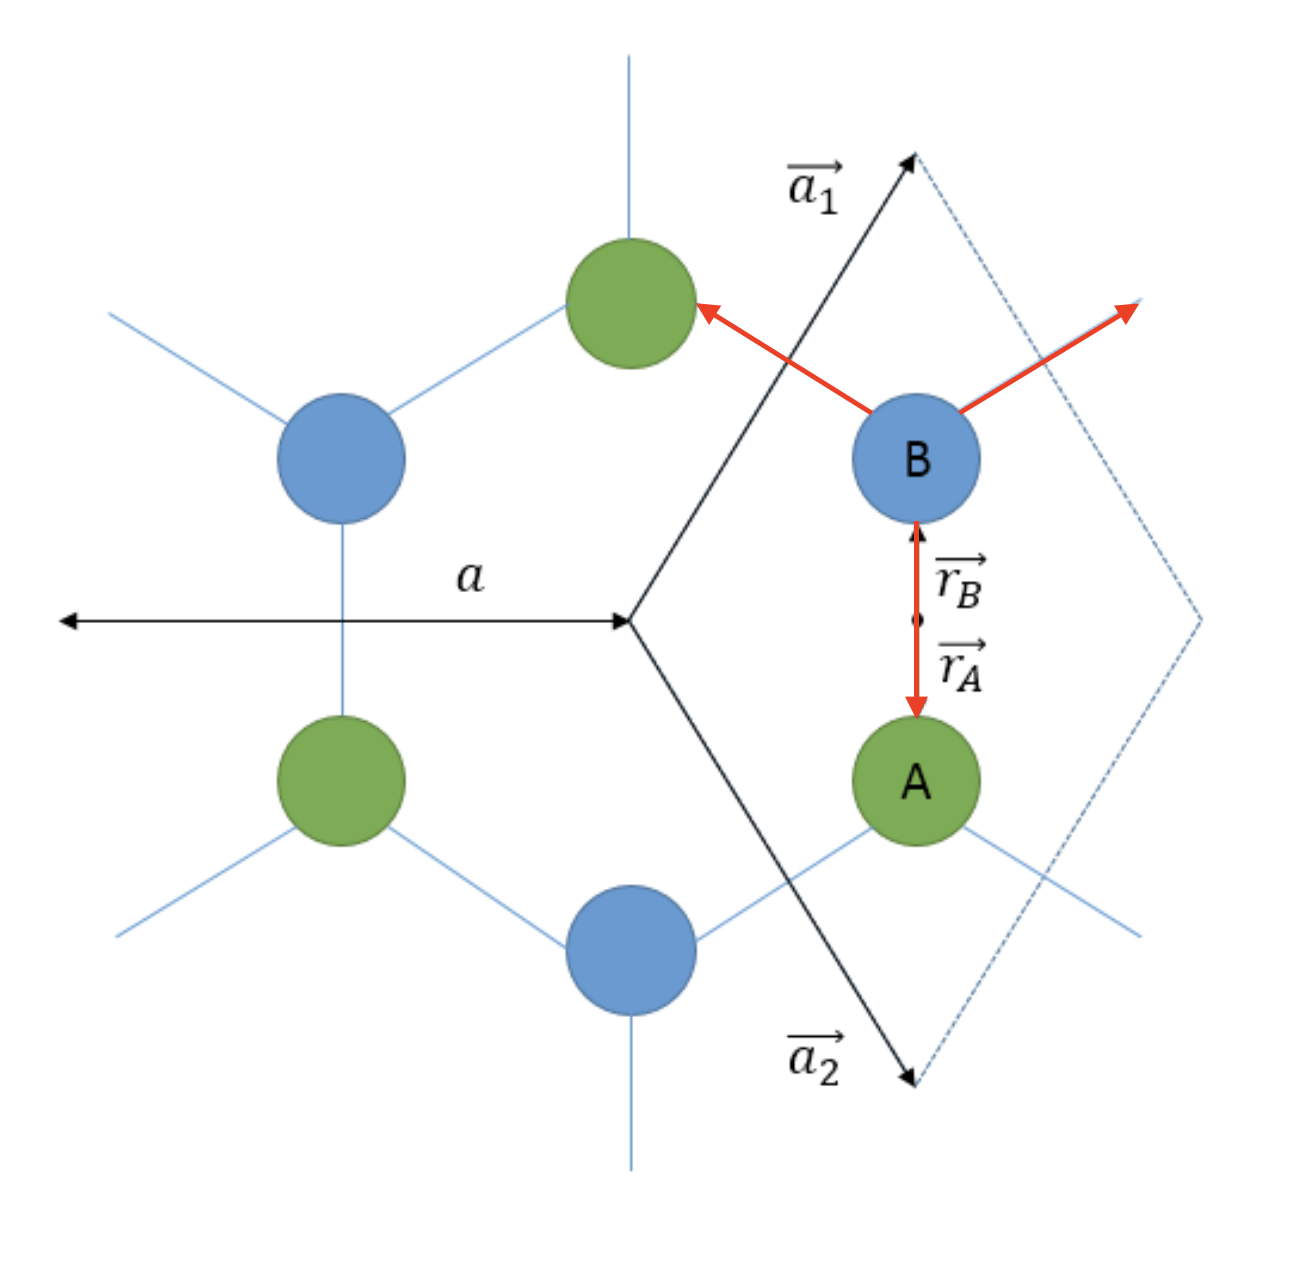
\includegraphics[scale=.42]{nearest_neighbor1}
\caption{The monolayer configuration with the nearest neighbor lattice vectors $\vec{d}_{1}$, $\vec{d}_{2}$, $\vec{d}_{3}$ added in red. }
\end{figure}

To convert from a primitive lattice vector representation to a nearest neighbor vector representation, we can make use of the following
relationships.
$$\vec{a}_{1} = \vec{d}_{2} - \vec{d}_{3}$$
\begin{equation}
\vec{a}_{2} = \vec{d}_{3} - \vec{d}_{1}
\end{equation}

If we make this substitution, then our monolayer Hamiltonian becomes


\subsection{Reciprocal Lattice}
We may define a lattice point over some three-dimensional lattice as

\begin{equation}
\vec{R} = n_{1}\vec{a}_{1} + n_{2}\vec{a}_{2} + n_{3}\vec{a}_{3}
\end{equation}

where $\vec{a}_{i}$ are primitive lattice vectors. For example, in the case of
graphene, all lattice points can be constructed from the relation

\begin{equation}
\vec{R} = n_{1}\vec{a}_{1} + n_{2}\vec{a}_2 = n_{1}(\frac{a}{\sqrt{2}}, \frac{3a}{\sqrt{2}}) + n_{2}(\frac{a}{\sqrt{2}}, -\frac{3a}{\sqrt{2}})
\end{equation}
among others depending on the choice of primitive lattice vectors, which is not unique.
Now, in the reciprocal space, a point $\vec{G}$ on the reciprocal lattice may be defined to obey
\begin{equation}
e^{i\vec{G}\cdot\vec{R}} = 1
\end{equation}
where $\vec{G}$ can be similarly written as a function of primitive lattice vectors $\vec{b}_{i}$.
\begin{equation}
\vec{G} = m_{1}\vec{b}_{1} + m_{2}\vec{b}_{2} + m_{3}\vec{b}_{3}
\end{equation}
Since our relationship is well defined such that (where $\eta$ is some integer)
\begin{equation}
\vec{G}\cdot\vec{R} = \sum_{i}m_{i}n_{i}\vec{a}_{i}\cdot\vec{b}_{i} = 2\eta\pi
\end{equation}
then, if $m_{i}$ and $n_{i}$ are integers, then $\vec{a}_{i}\cdot\vec{b}_{i} = 2\pi$. In general, the primitive
reciprocal lattice vectors are defined such that
\begin{equation}
\vec{a}_{i}\cdot\vec{b}_{j} = \delta_{ij}
\end{equation}
It is also useful to consider the reciprocal lattice as a Fourier transform on the original lattice.
Generally speaking, a Fourier transform takes a function $f(x)$ and transforms it into a function of
the transform variable $\eta$. The form of the transformed function $\hat{f}(\eta)$ is
\begin{equation}
\hat{f}(\xi) = \int_{-\infty}^{\infty} f(x)e^{-2\pi ix\xi}dx
\end{equation}
We begin by considering a one-dimensional lattice, where the distance between lattice points is
given by $a$. Then, the lattice points are simply $R_{n} = an$. We could describe the lattice as a
density of lattice points:
\begin{equation}
\rho(r) = \sum_{n}\delta(r - an)
\end{equation}
In words, the collection of lattice points is described by a sum of delta functions that spike when the
position $r$ is equal to $an$, some integer multiple of $a$. Let's say we want to Fourier transform this
lattice density to obtain an expression in terms of $\vec{k}$, the wavevector. Then,

\begin{equation}
\hat{\rho}(k) = \int \rho(r)e^{-2\pi ikr}dr = \int \rho(r)e^{ikr}dr
\end{equation}
where in the last step we use $e^{-i2\pi} = 1$. This gives us
\begin{equation}
\hat{\rho}(k) = \sum_{n}\int \delta(r - an)e^{ikr}dr = \sum_{n}e^{ikan}
\end{equation}
In the last equation, a term in the sum is 1 if $k = \frac{2m\pi}{a}$, but all other k
values cancel out as the function is oscillatory. WHY???

\subsection{Brillouin Zones}
\begin{itemize}
\item A system which is periodic in real space with periodicity $a$ will be periodic in reciprocal
space with periodicity $\frac{2\pi}{a}$
\end{itemize}
A Brillouin zone is defined as a unit cell of the reciprocal lattice. Because the wavevector is
periodic with regard to shifts by the reciprocal lattice vector $\vec{G}$, $k + \vec{G}$, the reciprocal unit cell
contains all physically unique values for $k$ and each physically unique value appears only once within the unit cell. \par
The process for constructing the first Brillouin zone is as follows:
\begin{itemize}
\item Draw a reciprocal lattice vector from from $\vec{k} = 0$ to all neigboring reciprocal lattice points.
\item Draw a perpendicular bisector on the reciprocal lattice vectors. These bisectors form the Brillouin zone boundary.
\item All $\vec{k}$ points that can be reached from $\vec{k} = 0$ without crossing a Brillouin zone boundary are in the
 first Brillouin zone.
 \item If the previous steps are continued, all points that can be reached without crossing two boundaries are in the
  second Brillouin zone, and so forth.
\end{itemize}
The first Brillouin zone is continuous, but higher Brillouin zones are typically constructed with multiple pieces. Each Brillouin zone
covers the same area or volume and there are as many $\vec{k}$-states within a given Brillouin zone as there are unit cells in
the reciprocal lattice.




\begin{thebibliography}{9}
\bibitem{oxford}
Steven H. Simon.
\textit{Lecture Notes for Solid State Physics}.
Oxford University, 2012.

\bibitem{mccann}
Edward McCann, Mikito Koshino.
\textit{The electronic properties of bilayer graphene}.
arXiv:1205.6953, 2012.

\bibitem{schonen}
Christian Schonenberger.
\textit{Bandstructure of Graphene and Carbon Nanotubes: An Exercise in Condensed Matter Physics}.
2000.

\bibitem{kuzmenko}
Kuzmenko A B, Crassee I, van der Marel D, Blake P, and Novoselov K S. 2009
\textit{Phys. Rev. B} 80 165406

\end{thebibliography}



\end{document}
